%%%%%%%%%%%%%%%%%%%%%%%%%%%%%%%%%%%%%%%%%%%%%%%%%%%%%%%%%%%
%% Congratulations, you've made an excellent choice
%% of writing your Tampere University thesis using
%% the LaTeX system. This document attempts to be
%% as complete a template as possible to let you focus
%% on the most important part: the writing itself.
%% Thus the details regarding the visual appearance
%% and even structure have already been worked out
%% for you!
%%
%% I sincerely hope you will find this template useful
%% in completing your thesis project. I've tried to
%% add comments (followed by the % sign) to clarify
%% the structure and purpose of some of the commands.
%% Most of the magic happens in the file tauthesis.cls,
%% which you are more than welcome to take a look at.
%% Just refrain from editing it in the most crucial
%% versions of the thesis!
%%
%% I wish you and your thesis project the best of luck!
%% If this template causes you trouble along the way
%% or if you've any suggestions for improving it,
%% please be in contact through GitHub
%% (<URL HERE>)
%%
%% Yours,
%%
%% Ville Koljonen
%%
%% PS. This template or its associated class file don't
%% come with a warranty. The content is provided as is,
%% without even the implied promise of fitness to the
%% mentioned purpose. You, as the author of the thesis,
%% are responsible for the entire work, including the
%% provided material. No one else is liable to you for
%% any damage inflicted on you or your thesis, were it
%% caused by using this template or not.
%%%%%%%%%%%%%%%%%%%%%%%%%%%%%%%%%%%%%%%%%%%%%%%%%%%%%%%%%%%

%%%%% NOTICE %%%%%
%% Please read through the entire template
%% (files under ./tex) to find all instructions.
%% It is possible that the attached pdf files
%% do not include the latest information.
%%%%%%%%%%%%%%%%%%

%%%%% INSTRUCTIONS FOR COMPILING THE DOCUMENT %%%%%
%% Overleaf: just click Recompile.
%% Terminal:
%%  1. pdflatex main.tex
%%  2. makeindex -s main.ist -t main.glg -o main.gls main.glo
%%  3. biber main
%%  4. pdflatex main.tex
%%  5. pdflatex main.tex
%% Similar sequence of commands is also required
%% in LaTeX specific editors.
%%%%%%%%%%%%%%%%%%%%%%%%%%%%%%%%%%%%%%%%%%%%%%%%%%%

%%% Set PDF version before doing anything else.

%%% set-pdf-version.tex
%
% This file is loaded by main.tex before any other operations, so that PDF
% version is set correctly for accessibility features.
%

\RequirePackage{ifluatex}

\def\mypdfminorversion{6}

\ifluatex

    \directlua {
        if pdf.getminorversion() \string~= \mypdfminorversion then
            if (status.pdf_gone and status.pdf_gone > 0)
            or (status.pdf_ptr and status.pdf_ptr > 0)
            then
                tex.error("PDF version cannot be changed anymore.")
            else
                pdf.setminorversion(\mypdfminorversion)
            end
        end
    }

\else

    \pdfminorversion=\mypdfminorversion

\fi


%%%%% METADATA %%%%%
%
% Always keep the following metadata up to date! This is important for your
% PDF file to comply to accessibility standards. (And yes, this information
% must remain here, before \documentclass[...]{...}.)

\def\myfititle{Kuvaava otsikko}
\def\myentitle{A Descriptive title}
\def\myauthor{Firstname Lastname}
\def\myfisubtitle{Tarkentava alaotsikko}
\def\myensubtitle{A Specifying Subtitle}
\def\myfithesistype{Opinnäytetyön taso}
\def\myenthesistype{Thesis type}
\def\myexaminers{Title1 Firstname1 Lastname1 \\ Title2 Firstname2 Lastname2 \\ ...}
\def\myfifacultyname{Tiedekunnan nimi}
\def\myenfacultyname{The name of the faculty}
\def\myfiprogrammename{Tutkinto-ohjelman nimi}
\def\myenprogrammename{The name of the study programme}
\def\myfikeywords{avainsana1, avainsana2, ...}
\def\myenkeywords{keyword1, keyword2, ...}
\def\mylanguagecode{en-US}
\def\mysubject{A short description of the thesis subject.}
\def\myyear{2023}
\def\mymonth{06}
\def\myday{03}

%%%%% PREAMBLE %%%%%

%%%%% Document class declaration.
%
% The possible optional arguments are
%
%   finnish - thesis in Finnish (default)
%   english - thesis in English
%   numeric - citations in numeric style (default)
%   authoryear - citations in author-year style
%   apa - citations in APA 7 (available only in English)
%   ieee - citations in IEEE style (available only in English)
%   draft - for faster non-final works, also skips images
%           (recommended, remove in final version)
%   programs - if you wish to display code snippets
% Example: \documentclass[english, authoryear]{tauthesis}
%          thesis in English with author-year citations

\documentclass[finnish]{tauthesis}

%%% preamble.tex
%
% This file is for including LaTeX libraries or packages and defining your own
% commands.
%
% NOTE: The glossaries package loaded by tauthesis.cls throws a warning: No
% language module detected for 'finnish'. You can safely ignore this. All
% other warnings should be taken care of, before your thesis is submitted!

%%%%% Your packages.
%
% Before adding packages, see if they can be found in tauthesis.cls already.
% If you're not sure that you need a certain package, don't include it in the
% document! This can dramatically reduce compilation time.

% Graphs
% \usepackage{pgfplots}
% \pgfplotsset{compat=1.15}

% Subfigures and wrapping text
% \usepackage{subcaption}

%% Theorem environments and their numbering.
%
% Define both English and Finnish theorem types. These all follow the same
% counter. See the documentation of amsthm to see how these can be changed to
% suit your needs, if necessary.
%

\usepackage{amsthm}

\theoremstyle{definition}

\newtheorem{definition}{Definition}[chapter]
\newtheorem{theorem}[definition]{Theorem}
\newtheorem{lemma}[definition]{Lemma}
\newtheorem{corollary}[definition]{Corollary}
\newtheorem{example}[definition]{Example}

\newtheorem{maaritelma}[definition]{Määritelmä}
\newtheorem{lause}[definition]{Lause}
\newtheorem{apulause}[definition]{Apulause}
\newtheorem{seurauslause}[definition]{Seurauslause}
\newtheorem{esimerkki}[definition]{Esimerkki}

% Mathematics packages
\usepackage{mathtools, amssymb}
%\usepackage{bm}

% Chemistry packages
% \usepackage{chemfig}
% \usepackage[version=4]{mhchem}

% Text hyperlinking
% \usepackage{hyperref}
% \hypersetup{hidelinks}

% (SI) unit handling
\usepackage{siunitx}

\sisetup{
    detect-all,
    math-sf=\mathrm,
    exponent-product=\cdot,
    output-decimal-marker={,} % for theses in FINNISH!
}

%% For code listings.

\usepackage{listings}

% This global code listing configuration is required for automatically
% replacing special characters with corresponding LaTeX commands, in code files
% included with \lstinputlisting. Without it, letters like 'ä' in code file
% comments will result in a LaTeX errors.
%
% Source: https://tex.stackexchange.com/a/574950.

\lstset{
    inputencoding = utf8,  % Input encoding
    extendedchars = true,  % Extended ASCII
    literate      =        % Support additional characters
        {á}{{\'a}}1  {é}{{\'e}}1  {í}{{\'i}}1 {ó}{{\'o}}1  {ú}{{\'u}}1
        {Á}{{\'A}}1  {É}{{\'E}}1  {Í}{{\'I}}1 {Ó}{{\'O}}1  {Ú}{{\'U}}1
        {à}{{\`a}}1  {è}{{\`e}}1  {ì}{{\`i}}1 {ò}{{\`o}}1  {ù}{{\`u}}1
        {À}{{\`A}}1  {È}{{\`E}}1  {Ì}{{\`I}}1 {Ò}{{\`O}}1  {Ù}{{\`U}}1
        {ä}{{\"a}}1  {ë}{{\"e}}1  {ï}{{\"i}}1 {ö}{{\"o}}1  {ü}{{\"u}}1
        {Ä}{{\"A}}1  {Ë}{{\"E}}1  {Ï}{{\"I}}1 {Ö}{{\"O}}1  {Ü}{{\"U}}1
        {â}{{\^a}}1  {ê}{{\^e}}1  {î}{{\^i}}1 {ô}{{\^o}}1  {û}{{\^u}}1
        {Â}{{\^A}}1  {Ê}{{\^E}}1  {Î}{{\^I}}1 {Ô}{{\^O}}1  {Û}{{\^U}}1
        {œ}{{\oe}}1  {Œ}{{\OE}}1  {æ}{{\ae}}1 {Æ}{{\AE}}1  {ß}{{\ss}}1
        {ẞ}{{\SS}}1  {ç}{{\c{c}}}1 {Ç}{{\c{C}}}1 {ø}{{\o}}1  {Ø}{{\O}}1
        {å}{{\aa}}1  {Å}{{\AA}}1  {ã}{{\~a}}1  {õ}{{\~o}}1 {Ã}{{\~A}}1
        {Õ}{{\~O}}1  {ñ}{{\~n}}1  {Ñ}{{\~N}}1  {¿}{{?`}}1  {¡}{{!`}}1
        {°}{{\textdegree}}1 {º}{{\textordmasculine}}1 {ª}{{\textordfeminine}}1
        {£}{{\pounds}}1  {©}{{\copyright}}1  {®}{{\textregistered}}1
        {«}{{\guillemotleft}}1  {»}{{\guillemotright}}1  {Ð}{{\DH}}1  {ð}{{\dh}}1
        {Ý}{{\'Y}}1    {ý}{{\'y}}1    {Þ}{{\TH}}1    {þ}{{\th}}1    {Ă}{{\u{A}}}1
        {ă}{{\u{a}}}1  {Ą}{{\k{A}}}1  {ą}{{\k{a}}}1  {Ć}{{\'C}}1    {ć}{{\'c}}1
        {Č}{{\v{C}}}1  {č}{{\v{c}}}1  {Ď}{{\v{D}}}1  {ď}{{\v{d}}}1  {Đ}{{\DJ}}1
        {đ}{{\dj}}1    {Ė}{{\.{E}}}1  {ė}{{\.{e}}}1  {Ę}{{\k{E}}}1  {ę}{{\k{e}}}1
        {Ě}{{\v{E}}}1  {ě}{{\v{e}}}1  {Ğ}{{\u{G}}}1  {ğ}{{\u{g}}}1  {Ĩ}{{\~I}}1
        {ĩ}{{\~\i}}1   {Į}{{\k{I}}}1  {į}{{\k{i}}}1  {İ}{{\.{I}}}1  {ı}{{\i}}1
        {Ĺ}{{\'L}}1    {ĺ}{{\'l}}1    {Ľ}{{\v{L}}}1  {ľ}{{\v{l}}}1  {Ł}{{\L{}}}1
        {ł}{{\l{}}}1   {Ń}{{\'N}}1    {ń}{{\'n}}1    {Ň}{{\v{N}}}1  {ň}{{\v{n}}}1
        {Ő}{{\H{O}}}1  {ő}{{\H{o}}}1  {Ŕ}{{\'{R}}}1  {ŕ}{{\'{r}}}1  {Ř}{{\v{R}}}1
        {ř}{{\v{r}}}1  {Ś}{{\'S}}1    {ś}{{\'s}}1    {Ş}{{\c{S}}}1  {ş}{{\c{s}}}1
        {Š}{{\v{S}}}1  {š}{{\v{s}}}1  {Ť}{{\v{T}}}1  {ť}{{\v{t}}}1  {Ũ}{{\~U}}1
        {ũ}{{\~u}}1    {Ū}{{\={U}}}1  {ū}{{\={u}}}1  {Ů}{{\r{U}}}1  {ů}{{\r{u}}}1
        {Ű}{{\H{U}}}1  {ű}{{\H{u}}}1  {Ų}{{\k{U}}}1  {ų}{{\k{u}}}1  {Ź}{{\'Z}}1
        {ź}{{\'z}}1    {Ż}{{\.Z}}1    {ż}{{\.z}}1    {Ž}{{\v{Z}}}1
}

%%%%% Your commands.

% Print verbatim LaTeX commands
\newcommand{\verbcommand}[1]{\texttt{\textbackslash #1}}

% Command for formatting code.

\newcommand\code[1]{\texttt{#1}}

% A delimiter command for the norm of a vector with mathtools.

\DeclarePairedDelimiter\norm{\lVert}{\rVert}

% Basic theorems in Finnish and in English.
% Remove [chapter] if you wish a simply
% running enumeration.
% \newtheorem{lause}{Lause}[chapter]
% \newtheorem{theorem}[lause]{Theorem}

% \newtheorem{apulause}[lause]{Apulause}
% \newtheorem{lemma}[lause]{Lemma}

% Use these versions for individually
% enumerated lemmas
% \newtheorem{apulause}{Apulause}[chapter]
% \newtheorem{lemma}{Lemma}[chapter]

% Definition style
% \theoremstyle{definition}
% \newtheorem{maaritelma}{Määritelmä}[chapter]
% \newtheorem{definition}[maaritelma]{Definition}
% examples in this style

%%%%% Glossary information.

% Use the following lines ONLY if you need more
% than one glossary. The first argument specifies
% a type label for the glossary and the second
% the displayed name.
% \newglossary*{symbs}{Symbols}
% \newglossary{label}{Displayed name}
% ...

\makeglossaries

% Use this line if using the default glossary.
% Otherwise comment out.

\loadglsentries[main]{tex/sanasto.tex}

% Use this line if using more than one glossary.
% Otherwise comment out.
% \loadglsentries[symbs]{tex/sanasto2.tex}

%%%%% Citation information.

% Commonly used bibliography modifications.
% Feel free to play around with them.

%\ExecuteBibliographyOptions{%
%sorting=none,
%maxbibnames=99,
%maxcitenames=2,
%giveninits=true,
%uniquename=init,
%sortcites,
%sortlocale=fin}

%\DeclareNameAlias{sortname}{last-first}
%\DeclareNameAlias{author}{last-first}

%\DeclareFieldFormat[%
%    article,inbook,incollection,inproceedings,
%    patent,thesis,unpublished]{citetitle}{#1\isdot}
%\DeclareFieldFormat[%
%    article,inbook,incollection,inproceedings,
%    patent,thesis,unpublished]{title}{#1\isdot}
%\DeclareFieldFormat{pagetotal}{#1 \bibstring{page}}

%\AtBeginBibliography{\renewcommand*{\makelabel}[1]{#1\hss}}

%\DefineBibliographyExtras{english}{\let\finalandcomma=\empty}

\addbibresource{tex/references.bib}
 % You can add packages and define new commands in this file.

\begin{document}

%%%%% FRONT MATTER %%%%%

\frontmatter

%%%%% Thesis information and title page.

% Enable the use of @ character in command names.

\makeatletter

% The titles of the work. If there is no subtitle, leave the \myfisubtitle or
% \myensubtitle command arguments empty. Pass the title in the primary
% language as the first argument and its translation to the secondary language
% as the second.

\if@langenglish

    \title{\myentitle}{\myfititle}

\else

    \title{\myfititle}{\myentitle}

\fi

\if@langenglish

    \subtitle{\myensubtitle}{\myfisubtitle}

\else

    \subtitle{\myfisubtitle}{\myensubtitle}

\fi

% The author name.

\author{\myauthor}

% The examiner information. If your work has multiple examiners, replace with
%
%   \examiner[<label>]{<name> \\ <name>}
%
% where <label> is an appropriate (plural) label, e.g. Examiners or
% Tarkastajat, and <name>s are replaced by the examiner names, each on their
% separate line.

\examiner{\myexaminers}

% The finishing date of the thesis (YYYY-MM-DD).

\finishdate{\myyear}{\mymonth}{\myday}

% The type of the thesis (e.g. Kandidaatintyö or Master of Science Thesis) in
% the primary and the secondary languages of the thesis.

\if@langenglish

    \thesistype{\myenthesistype}{\myfithesistype}

\else

    \thesistype{\myfithesistype}{\myenthesistype}

\fi

% The faculty and degree programme names in the primary and the secondary
% languages of the thesis, respectively.

\if@langenglish

    \facultyname{\myenfacultyname}{\myfifacultyname}

\else

    \facultyname{\myfifacultyname}{\myenfacultyname}

\fi

\if@langenglish

    \programmename{\myenprogrammename}{\myfiprogrammename}

\else

    \programmename{\myfiprogrammename}{\myenprogrammename}

\fi

% The keywords of the thesis in the primary and the secondary languages of the
% thesis.

\if@langenglish

    \keywords{\myenkeywords}{\myfikeywords}

\else

    \keywords{\myfikeywords}{\myenkeywords}
\fi

% Make @ a regular letter again.

\makeatother

% Actually generate the title page based on the above commands.

\maketitle


%%%%% Abstracts and preface.
%
% Write the abstract(s) and the preface into a separate file for the sake of
% clarity. Pass the appropriate file name as the first argument to these
% commands. Put the \abstract in the primary language first and the
% \otherabstract in the secondary language second. Those who do not speak
% Finnish only need the first abstract. The second argument of the \preface
% command takes the place where the thesis was signed in.

\abstract{tex/tiivistelma.tex}

\otherabstract{tex/abstract.tex}

\preface{tex/alkusanat.tex}{Tampereella}

%%%%% Table of contents.

\tableofcontents

%%%%% Lists of figures, tables, listings and terms.
%
% Print the lists of figures and/or tables. Uncomment either of these commands
% as required. Both are optional, but if there are many important
% figures/tables, listing them may be a good idea.

% \listoffigures
% \listoftables
% \lstlistoflistings

% Misc stuff related to how the glossary is displayed. You can especially
% tweak the lengths to suit you!

\glsaddall
\setglossarystyle{taulong}
\setlength{\glsnamewidth}{0.25\textwidth}
\setlength{\glsdescwidth}{0.75\textwidth}
\renewcommand*{\glsgroupskip}{}

% Print the default glossary of abbreviations, if necessary. Otherwise comment
% out. The appropriate Finnish variant is 'Lyhenteet'

\printglossary[title={Lyhenteet ja merkinnät}]

% Print more than one glossary with these lines. Otherwise comment out.

% \printglossary[type=symbs]
% \printglossary[type=label]
% ...

%%%%% MAIN MATTER %%%%%

\mainmatter

% Write each of the chapters of the thesis into a separate file for the sake
% of clarity. They can be \input as shown below. Give both the chapters and
% their files as descriptive names as possible.

\chapter{Johdanto}%
\label{ch:johdanto}

Koneoppimisella voidaan hakea ratkaisua monenlaisiin ongelmiin. Sen avulla voidaan pyrkiä ratkaisemaan normaalisti erittäin monimutkaisia algoritmeja vaativia ongelmia. Käytännössä mikä tahansa tietotekninen ongelma on teoriassa ratkaistavissa koneoppimisella. Se ei kuitenkaan aina ole tarpeellinen tai mahdollinen ratkaisu. Tarpeettoman monimutkaisuuden sekä ”black box” ongelmien välttelyn ohella, yhtenä suurimpana esteenä sen toteuttamisessa on hyvän koulutusdatan hankkiminen. Tämänhetkiset käyttökelpoiset mallit koulutetaan koulutusdatan avulla, ja nämä mallit voivat olla vain yhtä hyviä kuin niissä käytettävä koulutusdata.

Näin ollen jos halutaan luoda malli joka ei käytä yleisesti saatavilla olevaa koulutusdataa, hankaloituu sen luominen huomattavasti. Yleisimmin saatavilla olevat mallit ovat ihmisten sekä asioiden tunnistamiseen. Jos tavoittelemamme asia on variaatio tästä tai jostain muusta yleisestä mallista, voi uuden datan luomiseen alusta aloittamisen sijaan käyttää olemassa olevia malleja. Kuitenkin mitä kauemmas siirrytään selkeästä tehtävästä niin kuin objektin tunnistus, hankaloituu totuuden määrittäminen ja näin ollen myös hyvän ja toimivan mallin luominen.

Tässä työssä pyritään käyttämään segmentointi sekä syvyysdataa mallin luomiseen joka antaa syvyysdatan, ilman liikkuvia kohteita niin kuin autoja tai ihmisiä. Tämä pyritään saavuttamaan mahdollisimman automaattisesti, ja tavalla joka on hyödynnettävissä mahdollisimman geneerisesti eri mallien kanssa.

Lopullisen koulutusdatan generointiin tarvitaan siis tieto irtonaisista kohteista kuvassa, kuvan syvyysdata sekä jonkinlainen arvio tunnistetun kohteen takana olevasta alueesta. Paras keino tämän datan generointiin olisi kuvien manuaalinen läpikäynti ja syvyysdatan ”värittäminen” kuvaan. Tässä työssä kuitenkin pyritään työ tekemään mahdollisimman automaattisesti, resurssien säästämiseksi. Vaikka datan generointiin voidaankin käyttää pitkälti perinteisiä kuvankäsittely algoritmeja ei sen avulla todennäköisesti ole mahdollista tuottaa täysin luotettavaa dataa, koska kohteiden takana olevien asioiden tieto puuttuu stereokuvista. Tämän tiedon irrottaminen automaattisesti voisi olla mahdollista jos lähtökohtana käytettäisiin videokuvaa, mutta toteutettavan mallin kompleksisuus kasvaisi huomattavasti. Datasetin luominen alusta olisi myös mahdollista jos stereokameralla otettaisiin kuvia samasta kohteesta niin pitkällä aikavälillä että kaikki liikkuvat kohteet olisivat väistyneet. Tällaisen datasetin luominen tai löytäminen on kuitenkin hyvin hankalaa. 

Tällaista mallia voisi pidemmälle jalostettuna hyödyntää moniin eri käyttökohteisiin. Sitä voisi hyödyntää automatisoinnissa, kun tilasta saadaan helposti puhdas malli. Näin voidaan generoida esimerkiksi automaattiajamisessa käytettävät liikkeet suoraan tyhjään tilaan. Samaa voisi hyödyntää tilojen 3d skannauksessa. Ei olisi niin tarpeellista siivota tilaa ja jatkojalostuksella tunnistetut huonekalut tai muut siirrettävät asiat voitaisiin sisustaa suoraan generoituun pistepilveen tai 3d malliin. Tämä mahdollistaisi myös 3d skannauksen esimerkiksi peleissä, jolloin ympäristö voisi olla suoraan interaktiivinen, ilman niin suurta manuaalista työtä. 

Tässä työssä käytettävä data on itseajavien autojen kehitykseen liittyvää kaupunkidataa. Siitä löytyy valmiina, syvyysdata sekä segmentointidata. Kuitenkin koska mallin ja sen rakentamistyökalujen tulee olla hyödynnettävissä myös muulla datalla, käydään läpi myös stereokuvasta syvyysdatan hankinta, sekä segmentointimallin luonti. Lopputuloksessa käytetään kuitenkin, valmiiksi tarjottuja malleja segmentoinnin sekä syvyysdatan osalta.

Lopullisen tuotoksen olisi tarkoitus olla malli jolle tarjotaan stereokuva ja se palauttaa syvyysdatan ilman liikkuvia kohteita kuvassa.

\chapter{Esitystyyli}%
\label{ch:esitystyyli}

Tekstin sisällön lisäksi esitystyyli vaikuttaa suuresti viestinnän onnistumiseen. Ulkoasu ja kirjoitustyyli antavat työstä ja kirjoittajasta kuvan, toivottavasti hyvän.

\section{Teksti}

Älä suotta murehdi tekstin asettelusta, tämä pohja hoitaa sen jo valmiiksi. Kirjoitustyylin perusohjeet ovat:

\begin{itemize}
\item Ajattele lukijaa aina tekstiä kirjoittaessasi ja johdattele häntä riittävästi. Anna ensin yleiskuva ja liitä siihen yksityiskohdat.
\item Korosta tärkeimmät asiat, esimerkiksi nostamalla ne omiksi luvuikseen (\verbcommand{section}, \verbcommand{subsection}), poimimalla taulukkoon tai selittämällä kuvan avulla. Tekstissä käytä korostamiseen kursivointia (\verbcommand{emph}), mutta älä korosta liikaa.
\item Vältä pitkiä virkkeitä ja monimutkaisia lauserakenteita. Piste on paras välimerkki.
\item Suosi aktiivimuodossa olevia verbejä ja sijoita ne lauseen alkupuolelle. Älä kuitenkaan käytä yksikön 1. persoonaa (minä) kuin alkusanoissa.
\item Vältä kapulakielisiä ilmauksia ja ammattislangia. Sano asiat suoraan. Käytä vakiintunutta teknistä sanastoa, merkintöjä ja neutraalia asiatyyliä.
\item Lukujen ja alalukujen tulee olla vähintään kahden kappaleen mittaisia ja mielellään keskenään tasapainoisia. Kappale muodostuu aina useammasta kuin yhdestä virkkeestä.
\item Luvut ja alaluvut numeroidaan korkeintaan kolmannelle tasolle (\verbcommand{subsection}) asti, esimerkiksi 4.4.2. Pohja huolehtii tästäkin automaattisesti.
\item Lyhenteitä ei tulisi käyttää liikaa. Käytä lyhenteissä pieniä ja isoja kirjaimia johdonmukaisesti.
\end{itemize}

\section{Lauseympäristöt}

Tiedostossa \code{preamble.tex} on määritelty lauseympäristöjä matemaattisen
tekstin kirjoittamista varten. Näistä esimerkkeinä toimivat suomen- ja
englanninkieliset lauseet~\ref{lause:pythagoras} ja \ref{theorem:pythagoras}.

\begin{lause}[Pythagoraan lause]\label{lause:pythagoras}
    Suorakulmaisen kolmion sivujen \(a\), \(b\) ja \(c\) pituuksille on voimassa yhtälö
    \begin{equation}\label{yht:pythagoras}
        a^2 + b^2 = c^2\,,
    \end{equation}
    jos \(c\) on hypotenuusa.
\end{lause}

\begin{theorem}[Pythagorean theorem]\label{theorem:pythagoras}
    For the sides of a right triangle, \(a\), \(b\) and \(c\), the equation
    \begin{equation}\label{eq:pythagoras}
        a^2 + b^2 = c^2
    \end{equation}
    holds, if \(c\) is the hypotenuse.
\end{theorem}

Tällä hetkellä määritellyt ympäristöt ovat \code{maaritelma}, \code{lause},
\code{apulause}, \code{seurauslause} ja \code{esimerkki}, sekä vastaavat
englanninkieliset ympäristöt \code{definition}, \code{theorem}, \code{lemma},
\code{corollary} ja \code{example}. Näitä on suotavaa käyttää silloin, kun
tekstissä esitellään jokin tärkeä tulos tai määritelmä, johon tarvitsee
viitata myöhemmin. Liika lauseympäristöjen käyttö johtaa kuitenkin
listamaiseen Landaun kirjoitustyyliin, joka ei ole kovin helppolukuista, ja on
sopivaa vain referenssityylisissä teksteissä, joista vain haetaan faktoja.
Diplomityö ei ole tällainen tekstityyppi.


\section{Kuvat}

Kaikkiin kuviin täytyy viitata tekstissä. Kuvan avulla voidaan esittää tietoa tiiviissä muodossa, mutta kuvan täytyy olla merkityksellinen työn sisällön kannalta ja kuva täytyy selittää tekstissä. Viittaus on mielellään samalla sivulla kuin kuva tai sitä ennen. Kuvat ja taulukot numeroidaan ja sijoitetaan pääsääntöisesti sivun yläreunaan, oman harkinnan mukaan. \LaTeX{}issa tämä tapahtuu sijoittamalla \verbcommand{caption}-komentoa seuraavalle riville \verbcommand{label}-komennon, jonka argumentti on kyseisen kuvan (tai taulukon) yksikäsitteinen tunniste. Viittaaminen tapahtuu \verbcommand{ref}-komennolla, johon syötetään haluttu tunniste. Lukua ei saa aloittaa (eikä mielellään lopettaa) kuvalla, taulukolla, kaavalla tai luettelolla, vaan sen ympärillä on oltava tekstiä. Kuvateksti sijoitetaan kuvan alle.

Kuvan keskeinen sisältö on selitettävä tekstissä, jotta sen sanomasta ei jää epäselvyyttä. Analysointiohjelmistojen tuottamat kuvat vaativat useimmiten muokkausta, kuten kuvassa \ref{fig:huolittelu}. Kuvan tekstien on oltava luettavissa, ja niiden kooksi suositellaan samaa kuin muussa tekstissä, 11 pt. Pyri siihen, että myös harmaasävyissä tulostettu kopio on luettava ja selkeä. Suosi vektorimuotoisia kuvatiedostotyyppejä \texttt{.eps} ja \texttt{.pdf} (\LaTeX{} ei syö \texttt{.svg}-tiedostoja\ldots), sillä niitä voi skaalata helposti laadun heikkenemättä. \LaTeX{} sisältää myös erittäin ilmaisuvoimaisia paketteja vektorigrafiikan (\texttt{tikz}) \parencite{tikz} ja kuvaajien (\texttt{pgfplots}) \parencite{pgfplots} piirtämiseen. Kuvassa \ref{fig:pgf-esimerkki} esitetään esimerkki jälkimmäisen avulla luodusta kuvaajasta.

\begin{figure}
\centering
%\begin{subfigure}{0.49\textwidth}
\pdftooltip{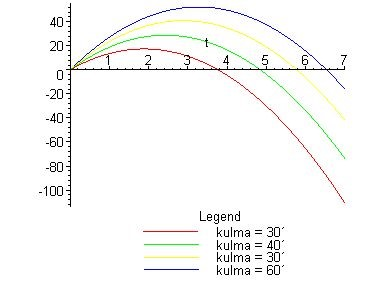
\includegraphics[width=\textwidth]{figures/bad-example.jpg}}{Kuva. Neljä alaspäin aukeavaa kaarta alkaa origosta eri lähtökulmilla. Kuvaajan skaalaus on huono ja akseleita ei ole nimetty johdonmukaisesti.}
%\end{subfigure}
%\begin{subfigure}{0.49\textwidth}
\pdftooltip{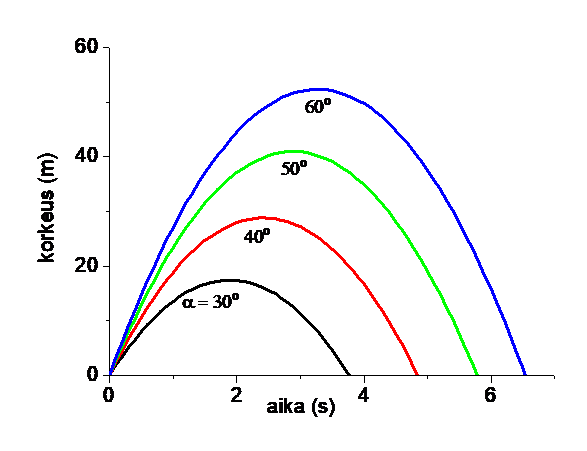
\includegraphics[width=\textwidth]{figures/good-example.png}}{Kuva. Neljä alaspäin aukeavaa kaarta alkaa origosta eri lähtökulmilla. Kuvaaja on skaalattu selkeäksi, akseleilla on täsmälliset nimet ja jokaiseen kuvaajaan liittyvä lähtökulmatieto on merkitty sen viereen.}
%\end{subfigure}
\caption[Tämä on lyhyt kuvateksti.]{Kuvaaja on hyvä muokata julkaisukelpoiseksi. Vasemmalla on esitetty muokkaamaton kuvaaja ja oikealla muokattu.}
\label{fig:huolittelu}
\end{figure}

\begin{figure}
\centering
%\input{figures/pgf-example.tex}
\caption{Kuvan \ref{fig:huolittelu} tyylinen esimerkki \texttt{pgfplots}-paketilla piirrettynä.}
\label{fig:pgf-esimerkki}
\end{figure}

\section{Taulukot}

Taulukot sopivat hyvin erityisesti numeerisen informaation esittämiseen tiiviissä muodossa. Kuvien tapaan taulukot numeroidaan ja varustetaan otsikolla, kuten taulukossa. Taulukkoteksti sijoitetaan samalle sivulle taulukon kanssa ja taulukon yläpuolelle. Suureet, lyhenteet ja symbolit selitetään tarvittaessa tekstissä. Kaikkiin taulukoihin on viitattava tekstissä, mieluummin ennen taulukkoa. Taulukon keskeinen sanoma ja tulkintaohjeet selitetään tekstissä.

Taulukon sarakkeet otsikoidaan, ja suureet sekä yksiköt laitetaan näkyviin. Jos otsikkoriviä tarvitsee erottaa muusta taulukosta, tee se korostamalla (\verbcommand{emph}). Taulukon järjestyksellä on suuri merkitys. Jokaista solua ei pidä ympäröidä reunaviivalla, koska taulukosta tulee raskaslukuinen. Lisää vaakaviiva taulukon ylä- ja alareunaan. Vaakaviivoja voi käyttää esimerkiksi 4--5 rivin välein, ellei tietoja muuten ole jaettu kategorioihin tai selkeys sitä vaadi. Sarakkeen numeroarvot tasataan desimaalipilkun kohdalta, jolloin arvoja on helppo vertailla. Tämä tapahtuu \LaTeX{}issa helposti \texttt{siunitx}-paketin \parencite{siunitx} taulukkomateriaalin avulla. Tavoitteena on, että suureet ilmaistaan SI-yksikössä ja käytetään joko vakiintuneita etuliitteitä tai kymmenen potenssin muotoja siten, että ne voidaan laittaa otsikkoriville (katso tässäkin \texttt{siunitx}). Muutamia suosituksia taulukoiden ja kuvien käytöstä löydät lähteestä \parencite{pubadvice2009}.

\begin{table}
\centering
\caption{Esimerkki höyrystysolosuhteista kahdessa ohutkalvorakenteessa.}
\label{tab:taulukkoesimerkki}
% Making scarce use of table lines is recommended
% for clarity. Even the outer lines are generally
% not needed! Use the siunitx package provided
% S column type for easy decimal alignment.
%\begin{tabular}{c|S[table-format=3.1] S[table-format=1.2] S[table-format=2.1e-1] S[table-format=2.1] S[table-format=2.0]@{--}S[table-format=3.0] S[table-format=1.1]}
%    \hline
%    aine & {paksuus} & {korjauskerroin} & {paine} & {lämpötila} & \multicolumn{2}{c}{virta} & {nopeus} \\[-0.5ex]
    % The syntax \\[<length>] inserts a vertical
    % space of <length> in addition to the normal
    % new line action provided by \\. This should
    % apply in any situation.
%    & {(\si{\nano\metre})} & & {(\si{\milli\bar})} & {(\si{\degreeCelsius})} & \multicolumn{2}{c}{(\si{\milli\ampere})} & {(\si{\nano\metre\per\second})} \\\hline
%    SiO2 & 181.0 & 1.10 & 3.0e-5 & 90.6 & 20 & 23 & 0.2 \\
%    TiO2 & 122.1 & 1.55 & 15.0e-5 & 91.1 & 93 & 100 & 0.1 \\\hline
%\end{tabular}
\end{table}

\section{Matemaattiset merkinnät ja yhtälöt}

Käytä selvyyssyistä mieluummin numeroita kuin kirjaimia lukuarvoissa: esimerkiksi ''6 työvaihetta'' on selkeämpi ja parempi kuin ''kuusi työvaihetta''. Tuhaterottimen käyttö selkeyttää tekstiä, eli kirjoita 55~700~125 muodon 55700125 sijaan. Desimaalipilkkua edeltävä nolla tulee aina merkitä. Suomen kielessä käytetään virallisesti desimaalipilkkua, englannin kielessä desimaalipistettä. Näistäkin tämä pohja ja \texttt{siunitx} \parencite{siunitx} huolehtivat siististi, jos vain annat niiden (muista ottaa \texttt{siunitx} käyttöön).

Numeroiden tavoin myös mittayksiköt kannattaa kirjoittaa lyhenteinä. Mittayksikön ja numeroarvon välissä on itse asiassa välilyöntiä lyhyempi väli, ja niiden tulee olla samalla rivillä. Taulukko tai kaavio on parempi esitystapa, jos tekstin sekaan tulee runsaasti numeroarvoja. Usein numeroarvoihin voi liittää laadullisen määreen, ja vastaavasti kaikkiin laadullisiin määreisiin (suuri, pieni, kallis, nopea) tulisi liittää numeroarvo kuvaamaan suuruusluokkaa. Numeroiden kanssa ei tarvitse käyttää sijapäätettä, jos seuraava sana on samassa sijassa (taivutusmuodossa), esimerkiksi ''jakautuu 10 osaan'' ja ''20 ja 50 sentin kolikot''. On myös tapauksia, joissa sijapääte pitää merkitä, esimerkiksi lauseessa ''osallistujia oli 7:stä eri maasta''.

Tekstissä tulee ensisijaisesti käyttää yleisesti tunnettuja ja hyvin määriteltyjä käsitteitä, joiden kirjoittamiseen on yleensä jokin vakiintunut merkintätapa tai symboli. Uudet käsitteet ja merkinnät pitää määritellä, kun ne esiintyvät tekstissä ensimmäisen kerran. Symboleissa ja mittayksiköissä isot ja pienet kirjaimet tarkoittavat eri asioita. Samaa symbolia ei tule käyttää monessa eri merkityksessä. Mittayksiköt merkitään selvästi.

Matemaattiset merkit ja kreikkalaiset kirjaimet löytyvät \LaTeX{}in makroista ja kaavamoodeista, kuten \(\Theta(n^2)\). Yksinkertaiset kaavat voivat olla osa virkettä (siis tekstiä) ja ilman numeroa. Esimerkkinä tekstistä erotetusta kaavasta Newtonin 2. peruslaki voidaan ilmaista muodossa
\begin{equation}\label{eq:newton2}
    m\mathbf{a} = \mathbf{F} \,,
\end{equation}
missä \(m\) on kappaleen massa, \(\mathbf{a}\) sen kiihtyvyys ja \(\mathbf{F}\) siihen kohdistuva nettovoima. Huomaa, että symbolien merkitys selitetään aina heti kaavan yhteydessä sillä tavalla kuin on luontevinta. Kaavat esitetään tarkoituksella eri fontilla ja matemaattiset symbolit pääosin kursivoidaan. Vektorit voidaan esittää lihavoituna, kuten edellä (tavallisinta painetussa tekstissä) tai nuolella varustettuna, kuten \(\vec{v}\). Dimensiollisia lukuja voidaan esittää \verbcommand{SI}-komennon avulla:
\begin{equation*}
    \norm{\mathbf{F}}
    =
    m\norm{\mathbf{a}}
    =
    \SI{10}{\kilogram} \cdot \SI{9.81}{\metre\per\second\squared}
    =
    \SI{98.1}{\newton} \,.
\end{equation*}

Matemaattinen kaava numeroidaan, jos se on omalla rivillään ja siihen viitataan muualla tekstissä, katso esimerkiksi kaava \eqref{eq:newton2}. Usein numero on tavallisten sulkujen sisällä ja tasattu oikeaan laitaan, kuten tässä ohjeessa. Matematiikan kirjoitusohjeiden ja englatilaisen kulttuuripiirin tavan mukaisesti kaavoihin sisällytetään välimerkit, kuten yhtälössä \eqref{eq:newton2} lopun pilkku. Toisinaan matemaattisen rakenteen edessä on tunniste, kuten Määritelmä 1 tai Lause 1 \parencite{matohje2009}. Nämä luodaan omilla \texttt{amsthm}-pakettiin pohjautuvilla ympäristöillään. Kaavojen ja muiden rakenteiden numerointi voi olla juokseva läpi koko tekstin ((1), (2), \ldots) tai aina yhden luvun sisällä ((1.1), (1.2), \ldots, (2.1), \ldots).

Älä aloita uutta virkettä matemaattisella symbolilla. Yleensä teknis-fysikaalisessa tekstissä kursivoidaan muuttujat, kuten \(x\) ja \(y\). Kursivoinneissa kannattaa luottaa \LaTeX{}in automatiikkaan \parencite{notsoshort}. Sen sijaan alkeisfunktioita, erikoisfunktioita ja operaattoreita merkitään tavallisella kirjasimella: \(\sin(2x + y)\) tai
\begin{equation*}
    \lim_{x \rightarrow -1}\frac{x^2 - 1}{x + 1} = -2 \,.
\end{equation*}
Kappaletta, tai varsinkaan lukua ei ole hyvä myöskään lopettaa kaavaan, kuvaan tai taulukkoon.

%Kemian symboleita tarvitseviakaan \LaTeX{} ei jätä pulaan. Molekyylikaavoja ja reaktioyhtälöitä, kuten \ce{CH3CH2CH2COOH} ja
%\begin{center}
%    \ce{N2 (g) + 3 H2 (g) <=> 2 NH3 (g)}
%\end{center}
%varten tarvitaan \texttt{mhchem}-paketti \parencite{mhchem}, ja kokonaisia rakennekaavoja varten \texttt{chemfig} \parencite{chemfig}. Esimerkkinä jälkimmäisestä voidaan esittää telluriumtetrafluoridin (\ce{TeF4}) Lewisin rakenne.
%\begin{center}
%    \chemfig{\lewis{0:,Te}
%    (-[:90]\lewis{0:2:4:,F})
%    (-[:270]\lewis{0:4:6:,F})
%    (<:[:135]\lewis{1:3:5:,F})
%    (<[:225]\lewis{3:5:7:,F})
%    }
%\end{center}
%Varsinkin rakennekaavojen latominen vaatii totuttelemista, mutta keinot ovat olemassa.

\section{Ohjelmat ja algoritmit}

Koodin kirjasinlajina käytetään \texttt{tasalevyistä kirjasinlajia}, jonka merkit ovat yhtä leveitä. Kun ohjelmakoodin tai algoritmin pituus on alle 10 riviä eikä siihen enää myöhemmin tekstissä viitata, se voidaan esittää kuten kaavat. Pidemmät, alle sivun mittaiset ohjelmakoodit tai algoritmit kirjoitetaan kuten Ohjelma \ref{prog:esimerkki}, otsikkona ''Ohjelma'' tai ''Algoritmi''.

Koodiin on hyvä lisätä muutamia kommentteja ja sisentää se johdonmukaisesti. Koodin toiminta selitetään aina myös juoksevassa tekstissä pääpiirteissään, lähinnä siitä esitetään muutamia avainhuomioita. Esimerkiksi \LaTeX{}in paketti \texttt{listings} \parencite{listings,notsoshort} osaa kätevästi sisällyttää sekä oikeita kooditiedostoja että pseudokoodia tekstiin, lisätä automaattisesti rivinumeroinnin ja korostaa monet varatut sanat. Käytä sitä kaiken koodin esittämiseen \LaTeX{}in avulla.

\renewcommand{\lstlistingname}{Ohjelma}
\lstinputlisting
    [
        float,
        caption={Esimerkki ohjelmakoodin esittämisestä.},
        label=prog:esimerkki,
        language=C,
        numbers=left,
        morekeywords={Kirjainpari},
        inputencoding=utf8,
    ]
    {code/esimerkkikoodi.c}

\section{Saavutettava opinnäytetyö}

Suomen laki vaatii Euroopan unionin saavutettavuusdirektiivin 2016/2102 mukaisesti, että sähköiseistä julkaisuista tehdään saavutettavia (järkevällä työmäärällä). Tämä pätee myös opinnäytetyöhösi, minkä vuoksi on hyvä tietää tai ottaa selvää työsi saavutettavuusvaatimuksista. Opinnäytetyön pohjan kirjoittaja tai ylläpitäjä ei ota minkäänlaista vastuuta puolestasi!

Tämä pohja pyrkii auttamaan lopullisen dokumentin saavutettavuuden parantamisessa niin paljon kuin mahdollista. Valitettavasti vuonna 2021 (ja luultavasti vuoteen 2024 asti) \LaTeX{} ei pysty tuottamaan PDF/UA standardin, tai edes hiukan vähemmän vaativien yliopiston ohjeiden mukaista tiedostoa. Pääsyynä on, että \LaTeX{} heittää muistin säästämiseksi paljon tähän tarvittavasta dokumentin rakenneinformaatiosta romukoppaan heti, kun mahdollista (muistiongelma oli todellinen 80- ja 90-luvuilla). Kaikkea toivoa ei kuitenkaan ole menetetty, ja työssä pitäisi silti pyrkiä maksimoimaan saavutettavuus!

Kuten opinnäytetyön ulkoasun kanssa, tämä pohja pyrkii automatisoimaan monet saavutettavuusratkaisut puolestasi. Muutamat seikat, joihin pitää kiinnittää huomiota kirjoittaessa ovat
\begin{enumerate}
\item selkeän ja merkitykseltään yksikäsitteisen kielen käyttäminen, sekä keskeisen informaation välittäminen sanoin, eikä vain visuaalisin keinoin,
\item vaihtoehtoisten tekstien (tekstivastineiden, alt-tekstien) kirjoittaminen \emph{kaikille} työssä käyttämillesi kuville,
\item dokumentin metadatakentistä otsikon ja pääkielen ylläpitäminen,
\item matematiikan automaattisen tekstivastineratkaisun kannalta yhteensopivien matematiikkaympäristöjen käyttäminen.
\end{enumerate}
Noudata näissä kohdissa seuraavia ohjeita.
\begin{enumerate}
\item Tee kuten yllä kuvattiin. Käytä tarvittaessa ulkoisia palveluja tekstisi helppolukuisuuden arvioimisen tukena.
\item Käytä komentoa \texttt{\textbackslash pdftooltip\{\ldots\}\{\ldots\}} paketista \texttt{pdfcomment} (sisältyy pohjaan).
\begin{verbatim}
\begin{figure}
\pdftooltip{\includegraphics[...]{...}}%
{Kuva. Tämä vaihtoehtoinen teksti kuvailee,
mitä näkevä käyttäjä näkee kuvassa.}
\caption{Kuvaotsikko}
\label{fig:jokulabeli}
\end{figure}
\end{verbatim}
Huomaa, että kuvaotsikko ja tekstivastine kirjoitetaan palvelemaan eri tarkoituksia ja että tekstivastine ei koskaan saa olla vain kuvaotsikon kopio! (Ruudunlukijat sitä paitsi lukevat kuvaotsikot tekstivastineen lisäksi.) Kuvaile tekstivastineessa kuvan visuaalista sisältöä runsaasti, mutta keskity myös vain olennaisimpiin merkityksiin, joita kuva välittää.
\item Pidä dokumentin metadatakentät aivan \texttt{main.tex}-tiedoston alussa aina ajan tasalla.
\item Älä käytä vanhoja \TeX{}-tyylisiä \verb+$...$+- ja \verb+$$...$$+-ympäristöjä matematiikkaa varten. Käytä niiden sijaan \LaTeX{}-tyylisiä \verb+\(...\)+- ja \verb+\[...\]+-ympäristöjä. Keskitetyn matematiikan tupladollareita ei muutenkaan pitäisi käyttää.

Suurin osa \texttt{amsmath}-paketin matematiikkaympäristöistä, kuten \texttt{equation}, \texttt{equation*} ja \texttt{align} saavat tekstivastineet automaattisesti oikein. Vastaavasti muissa paketeissa määriteltyjä matematiikkaympäristöjä ei tueta! Matematiikan tekstivastine kaikissa matematiikkaympäristöissä on yksinkertaisesti sen \LaTeX{}-lähdekoodi, kunnes parempi ratkaisu saadaan aikaiseksi.
\end{enumerate}


\chapter{Viittaustekniikat}%
\label{ch:viittaustekniikat}

Viittaus sisältää kaksi pääkohtaa: tekstissä esiintyvän lähdeviitteen ja lähdeluettelon, jossa on jokaisen lähteen yksilöivät (bibliografiset) tiedot. Tässä osiossa esitellään 2 yleistä viittausten merkintätapaa:
\begin{enumerate}
    \item numeroviittausjärjestelmä (Vancouver-järjestelmä), esim. [1], [2], \ldots
    \item nimi-vuosijärjestelmä (Harvard-järjestelmä), esim. (Weber 2001), (Kaunisto 2003), \ldots
\end{enumerate}
Numeroviittaus sijoitetaan hakasulkeisiin ja nimi-vuosiviittaus kaarisulkeisiin. Ensin mainitussa käytetään juoksevaa numerointia ja jälkimmäisessä tekijän sukunimeä ja julkaisuvuotta. Kumpikin viittaustapa on sallittu, ja niiden yleisyys vaihtelee aloittain. Valitse yksi ja ole järjestelmällinen sitä käyttäessäsi.

\LaTeX{}in tavallisimmin käytetty lähdeviittaustoiminto on pitkään ollut Bib\TeX. Se on kuitenkin jo vanha, ja sitä joustavampi ja ilmaisuvoimaisempi vaihtoehto on Bib\LaTeX{} \parencite{biblatex}. Käytännössä suuri osa tieteellisestä julkaisemisesta hyödyntää vanhempaa työkalua, mutta muutostakin on tapahtumassa. Näistä syistä tämä pohja ohjaa käyttämään Bib\LaTeX{}ia.

Molemmat esitellyt järjestelmät perustuvat siihen, että käytettyjen lähteiden bibliografiset tiedot kerätään \texttt{.bib}-tiedostoon erityisellä syntaksilla. Ohjelma lukee sekä tämän ''tietokannan'' että kirjoitettavan dokumentin, sekä muodostaa viitteet ja viiteluettelon niiden pohjalta. Seuraavassa käydään läpi molempien viittaustyylien muodostaminen Bib\LaTeX{}in avulla. Oletuksena pohjassa on aktiivisena numeroviittaus, ja sen voi vaihtaa nimi-vuosi\-järjestelmään kirjoittamalla dokumenttiluokan valinnaiseksi argumentiksi \texttt{authoryear}.

\section{Lähdeviittaukset tekstissä}

Lähdeviittaus sijoitetaan tekstin joukkoon mahdollisimman lähelle viittauskohtaa. Pääsääntönä tekstiviittaus sijoitetaan virkkeen sisälle ennen pistettä.

\begin{quotation}
\noindent Weber väittää, että\ldots [1].

\noindent Cattaneo et al. esittävät tutkimuksessaan [2] uuden\ldots

\noindent Tuloksena on\ldots [1, s. 23]. Pitää myös huomata\ldots [1, ss. 33--36]

\noindent Esitetyn teorian mukaan\ldots (Weber 2001).

\noindent Erityisesti on huomioitava\ldots (Cattaneo et al. 2004).

\noindent Weber (2001, s. 230) on todennut\ldots

\noindent Alan kirjallisuudessa [1, 3, 5] esitetyn mukaan\ldots

\noindent Alan kirjallisuudessa [1][3][5] esitetyn mukaan\ldots

\noindent Aihetta on tutkittu ja raportoitu erittäin laajasti [6--18]\ldots

\noindent\ldots kirjallisuudessa (Weber 2001; Kaunisto 2003; Cattaneo et al. 2004) on esitetty\ldots
\end{quotation}

Lähdeluettelon pohjana toimivan \texttt{.bib}-tiedoston jokaista erillistä lähdettä varten varataan yksikäsitteinen tunniste, joka aloittaa tietojen esittelyn. Tunnisteet kannattaa valita mahdollisimman kuvaaviksi, sillä kaikki viittaukset tapahtuvat niiden avulla. Numeroviittausjärjestelmässä jokainen viittaus luodaan \verbcommand{cite}-komennolla: esimerkiksi \verbcommand{cite\{notsoshort\}}. Tämä tuottaa paikalleen vaikkapa merkinnän \cite{notsoshort}, riippuen lopullisesta lähdeluettelosta. Viittaukseen voidaan lisätä tietoja valinnaisten argumenttien avulla: esimerkiksi kirjoittamalla \verbcommand{cite[s. 30]\{notsoshort\}} tuottaa \cite[s. 30]{notsoshort} ja \verbcommand{cite[katso][s. 30]\{notsoshort\}} tuottaa \cite[katso][s. 30]{notsoshort}.

Nimi-vuosijärjestelmä on monimutkaisempi, sillä se sallii monenlaisia siteerausmahdollisuuksia, kuten yllä nähdään. Bib\LaTeX{}in toimintalogiikka pysyy kuitenkin samanlaisena, vain komennot vaihtuvat. Tärkeimmät viittauskomennot ovat \verbcommand{parencite}, \verbcommand{parencite*}, \verbcommand{citeauthor} ja \verbcommand{textcite}, jotka tuottavat tuloksinaan (Oetiker et al. 2018), (2018), Oetiker et al. ja Oetiker et al. (2018) samassa järjestyksessä.  Lisää komentoja voi etsiä dokumentaatiosta \parencite{biblatex}.

\section{Lähdeluettelo}

Lähteestä kerrotaan vähintään
\begin{itemize}
    \item tekijä(t),
    \item otsikko,
    \item julkaisuaika,
    \item julkaisija,
    \item sivunumerot (kirjat ja lehdet), sekä
    \item verkko-osoite,
\end{itemize}
jos ne tiedetään. Bib\LaTeX{} huolehtii tietojen järjestämisestä keskenään samalla tavalla. Järjestelmän käytössä on oleellista tietää myös lähteen tyyppi: lehtiartikkeli, kirja, konferenssijulkaisu, raportti ja patentti ovat vain esimerkkejä erilaisista mahdollisuuksista. Tämä tieto sisällytetään \texttt{.bib}-tiedostoon, ja muotoilu tapahtuu automaattisesti lähteen tyypin perusteella. Alla on esitetty malliksi lehtiartikkelin tietojen kirjoittaminen lähteeksi \texttt{.bib}-tiedostoon.

\texttt{
\begin{quotation}
    \noindent @article\{braams1991babel,\\
    title=\{Babel, a multilingual style-option system \\
    for use with \textbackslash LaTeX’s standard document styles\},\\
    author=\{Braams, Johannes L\},\\
    journal=\{TUGboat\},\\
    volume=\{12\},\\
    number=\{2\},\\
    pages=\{291--301\},\\
    year=\{1991\}\\
    \}
\end{quotation}
}

Opinnäytteissä lähdeluettelo kannattaa järjestää aakkosjärjestykseen ensimmäisen kirjoittajan sukunimen perusteella. Tämä tapahtuu tässä pohjassa automaattisesti. Erinomainen keino muodostaa yksittäinen lähde nopeasti on etsiä sille pohja Google Scholarin avulla. Se luo automaattisesti hyvän yritteen Bib\TeX{}in ja Bib\LaTeX{}in käyttöön. Dokumentaation lisäksi hyvä yhteenveto mahdollisista lähdetyypeistä ja niihin liittyvistä kentistä löytyy lähteestä \parencite{bibmanagement}.


% Add chapters similarly.

\chapter{Yhteenveto}%
\label{ch:yhteenveto}

\section{tekeekö datalla mitään }

\section{Kehitysehdotukset}

\section{muut käyttökohteet}


%%%%% Bibliography/references.

% Print the bibliography according to the information in ./tex/references.bib
% and the in-line citations used in the body of the thesis.

% \emergencystretch=2em
\printbibliography[heading=bibintoc]

%%%%% Appendices.

% Use only if it clarifies the structure of the document. Remember to
% introduce each appendix and its content.

\begin{appendices}

\chapter{Lähdekoodi}%
\label{ch:liite}

Lähdekoodi on saatavilla github repossa;

https://github.com/skoskosko/dippatyo

\end{appendices}

\end{document}
